\documentclass[11pt,preprint, authoryear]{elsarticle}

\usepackage{lmodern}
%%%% My spacing
\usepackage{setspace}
\setstretch{1.2}
\DeclareMathSizes{12}{14}{10}{10}

% Wrap around which gives all figures included the [H] command, or places it "here". This can be tedious to code in Rmarkdown.
\usepackage{float}
\let\origfigure\figure
\let\endorigfigure\endfigure
\renewenvironment{figure}[1][2] {
    \expandafter\origfigure\expandafter[H]
} {
    \endorigfigure
}

\let\origtable\table
\let\endorigtable\endtable
\renewenvironment{table}[1][2] {
    \expandafter\origtable\expandafter[H]
} {
    \endorigtable
}


\usepackage{ifxetex,ifluatex}
\usepackage{fixltx2e} % provides \textsubscript
\ifnum 0\ifxetex 1\fi\ifluatex 1\fi=0 % if pdftex
  \usepackage[T1]{fontenc}
  \usepackage[utf8]{inputenc}
\else % if luatex or xelatex
  \ifxetex
    \usepackage{mathspec}
    \usepackage{xltxtra,xunicode}
  \else
    \usepackage{fontspec}
  \fi
  \defaultfontfeatures{Mapping=tex-text,Scale=MatchLowercase}
  \newcommand{\euro}{€}
\fi

\usepackage{amssymb, amsmath, amsthm, amsfonts}

\def\bibsection{\section*{References}} %%% Make "References" appear before bibliography


\usepackage[round]{natbib}

\usepackage{longtable}
\usepackage[margin=2.3cm,bottom=2cm,top=2.5cm, includefoot]{geometry}
\usepackage{fancyhdr}
\usepackage[bottom, hang, flushmargin]{footmisc}
\usepackage{graphicx}
\numberwithin{equation}{section}
\numberwithin{figure}{section}
\numberwithin{table}{section}
\setlength{\parindent}{0cm}
\setlength{\parskip}{1.3ex plus 0.5ex minus 0.3ex}
\usepackage{textcomp}
\renewcommand{\headrulewidth}{0.2pt}
\renewcommand{\footrulewidth}{0.3pt}

\usepackage{array}
\newcolumntype{x}[1]{>{\centering\arraybackslash\hspace{0pt}}p{#1}}

%%%%  Remove the "preprint submitted to" part. Don't worry about this either, it just looks better without it:
\makeatletter
\def\ps@pprintTitle{%
  \let\@oddhead\@empty
  \let\@evenhead\@empty
  \let\@oddfoot\@empty
  \let\@evenfoot\@oddfoot
}
\makeatother

 \def\tightlist{} % This allows for subbullets!

\usepackage{hyperref}
\hypersetup{breaklinks=true,
            bookmarks=true,
            colorlinks=true,
            citecolor=blue,
            urlcolor=blue,
            linkcolor=blue,
            pdfborder={0 0 0}}


% The following packages allow huxtable to work:
\usepackage{siunitx}
\usepackage{multirow}
\usepackage{hhline}
\usepackage{calc}
\usepackage{tabularx}
\usepackage{booktabs}
\usepackage{caption}


\newenvironment{columns}[1][]{}{}

\newenvironment{column}[1]{\begin{minipage}{#1}\ignorespaces}{%
\end{minipage}
\ifhmode\unskip\fi
\aftergroup\useignorespacesandallpars}

\def\useignorespacesandallpars#1\ignorespaces\fi{%
#1\fi\ignorespacesandallpars}

\makeatletter
\def\ignorespacesandallpars{%
  \@ifnextchar\par
    {\expandafter\ignorespacesandallpars\@gobble}%
    {}%
}
\makeatother

\newenvironment{CSLReferences}[2]{%
}

\urlstyle{same}  % don't use monospace font for urls
\setlength{\parindent}{0pt}
\setlength{\parskip}{6pt plus 2pt minus 1pt}
\setlength{\emergencystretch}{3em}  % prevent overfull lines
\setcounter{secnumdepth}{5}

%%% Use protect on footnotes to avoid problems with footnotes in titles
\let\rmarkdownfootnote\footnote%
\def\footnote{\protect\rmarkdownfootnote}
\IfFileExists{upquote.sty}{\usepackage{upquote}}{}

%%% Include extra packages specified by user
\usepackage{booktabs}
\usepackage{caption}
\usepackage{longtable}

%%% Hard setting column skips for reports - this ensures greater consistency and control over the length settings in the document.
%% page layout
%% paragraphs
\setlength{\baselineskip}{12pt plus 0pt minus 0pt}
\setlength{\parskip}{12pt plus 0pt minus 0pt}
\setlength{\parindent}{0pt plus 0pt minus 0pt}
%% floats
\setlength{\floatsep}{12pt plus 0 pt minus 0pt}
\setlength{\textfloatsep}{20pt plus 0pt minus 0pt}
\setlength{\intextsep}{14pt plus 0pt minus 0pt}
\setlength{\dbltextfloatsep}{20pt plus 0pt minus 0pt}
\setlength{\dblfloatsep}{14pt plus 0pt minus 0pt}
%% maths
\setlength{\abovedisplayskip}{12pt plus 0pt minus 0pt}
\setlength{\belowdisplayskip}{12pt plus 0pt minus 0pt}
%% lists
\setlength{\topsep}{10pt plus 0pt minus 0pt}
\setlength{\partopsep}{3pt plus 0pt minus 0pt}
\setlength{\itemsep}{5pt plus 0pt minus 0pt}
\setlength{\labelsep}{8mm plus 0mm minus 0mm}
\setlength{\parsep}{\the\parskip}
\setlength{\listparindent}{\the\parindent}
%% verbatim
\setlength{\fboxsep}{5pt plus 0pt minus 0pt}



\begin{document}



\begin{frontmatter}  %

\title{Question 4: Flows analysis}

% Set to FALSE if wanting to remove title (for submission)




\author[Add1]{Jan-Hendrik Pretorius}
\ead{20713479@sun.ac.za}





\address[Add1]{Stellenbosch University}


\begin{abstract}
\small{
This report investigates the relationship between the past performance
of actively managed funds and their future fund flows. Utilizing a
dataset excluding Funds of Funds (FoF) and index funds, I calculate
3-year rolling returns to gauge past performance and then analyze how
these returns correlate with future fund flows across different time
lags.
}
\end{abstract}

\vspace{1cm}





\vspace{0.5cm}

\end{frontmatter}

\setcounter{footnote}{0}



%________________________
% Header and Footers
%%%%%%%%%%%%%%%%%%%%%%%%%%%%%%%%%
\pagestyle{fancy}
\chead{}
\rhead{Question 4: Flows analysis}
\lfoot{}
\rfoot{\footnotesize Page \thepage}
\lhead{}
%\rfoot{\footnotesize Page \thepage } % "e.g. Page 2"
\cfoot{}

%\setlength\headheight{30pt}
%%%%%%%%%%%%%%%%%%%%%%%%%%%%%%%%%
%________________________

\headsep 35pt % So that header does not go over title




\hypertarget{rolling-returns-analysis}{%
\section{Rolling Returns Analysis}\label{rolling-returns-analysis}}

I categorize funds based on their rolling returns into three performance
indicators: Top, Middle, and Bottom. This categorization allows us to
analyze patterns in fund flows relative to past fund performance. The
plot of 3-year rolling returns shows that top-performing funds (blue)
have the highest peaks and volatility, indicating potential higher risk
and return. Middle (orange) and bottom (green) categories exhibit less
variation and often overlap, suggesting more consistent but lower
performance. Periods of convergence among all categories hint at
market-wide impacts. Overall, the top funds show greater fluctuation
and, at times, distinct outperformance relative to others.

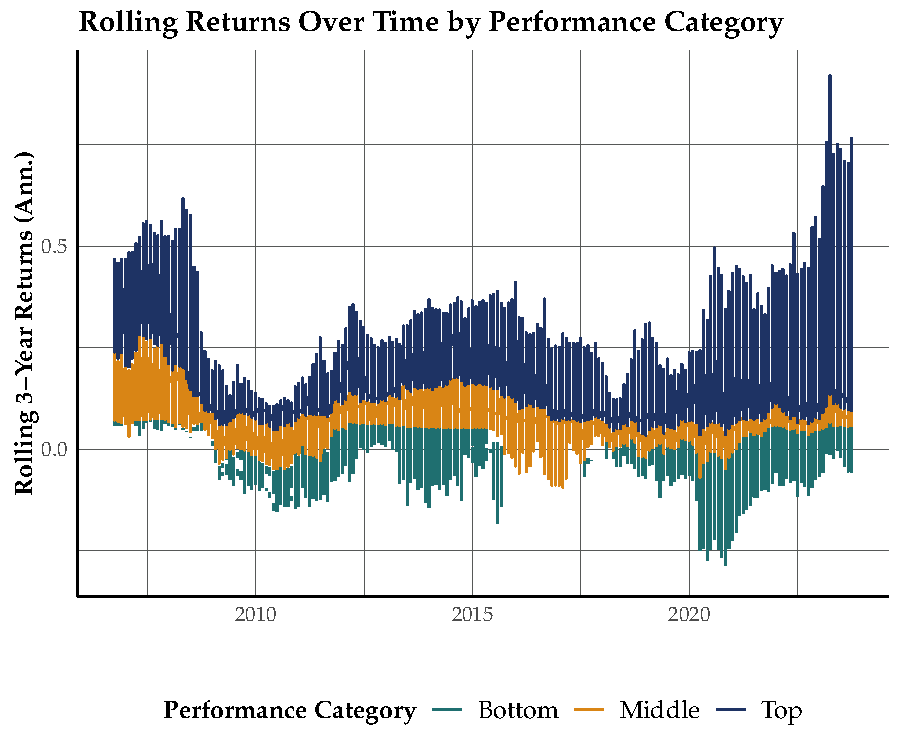
\includegraphics{Question-4_files/figure-latex/unnamed-chunk-1-1.pdf}

\hypertarget{fund-flows-analysis}{%
\section{Fund Flows Analysis}\label{fund-flows-analysis}}

Next, I compute future fund flows at various time lags (1 month, 6
months, 1 year, 2 years, and 3 years) to understand the lagged effect of
performance on investor behavior. I aggregate these flows by performance
category and observe the distribution of fund flows over time.

The plot below shows average fund flows by performance category over
time. The top-performing funds (blue) generally see positive inflows,
while the middle (orange) and bottom (green) categories exhibit more
variability with instances of both inflows and outflows. Notably, there
are periods where average flows for all categories decline, potentially
reflecting market downturns or investor sentiment shifts. The trend
lines suggest that top performers have a more consistent attraction of
funds, whereas middle and bottom performers experience more fluctuation
in investor contributions and withdrawals.

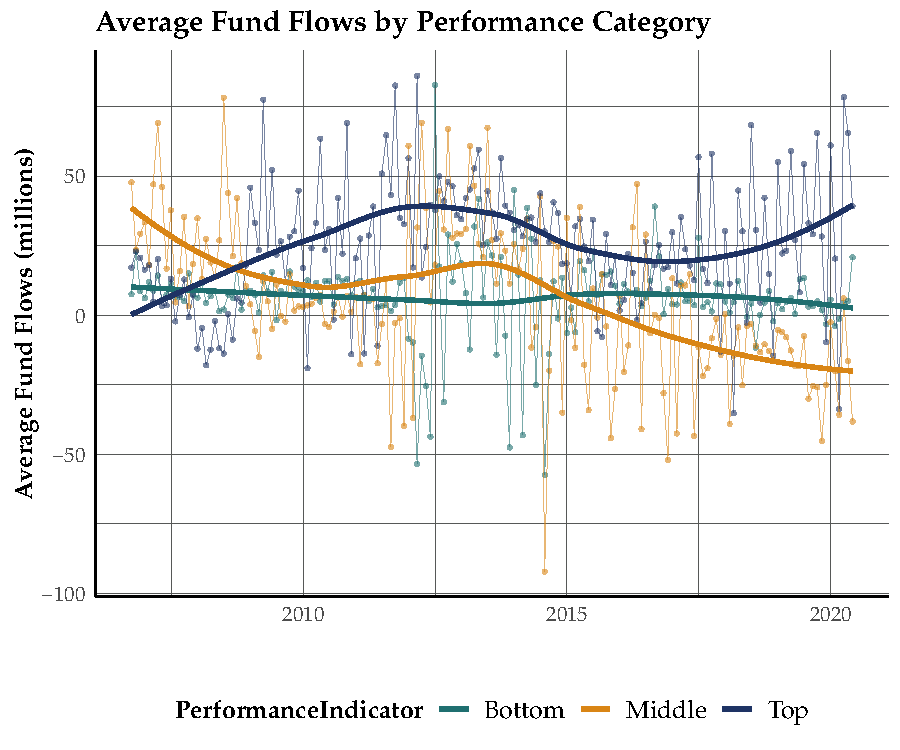
\includegraphics{Question-4_files/figure-latex/unnamed-chunk-2-1.pdf}

\hypertarget{correlation-analysis}{%
\section{Correlation Analysis}\label{correlation-analysis}}

To quantify the relationship between past performance and future flows,
I calculate correlation coefficients for each time lag. The results are
displayed in the table below, providing a clear presentation of the
correlation statistics, including confidence intervals and p-values.

\begin{longtable}{lrrrr}
\caption*{
{\large Correlation Between Rolling Returns and Future Fund Flows}
} \\ 
\toprule
Time Lag & Correlation & p-value & 95\% CI Lower & 95\% CI Upper \\ 
\midrule
Next Month & $0.038$ & $0.000$ & $0.031$ & $0.045$ \\ 
In 6 Months & $0.030$ & $0.000$ & $0.023$ & $0.037$ \\ 
Next Year & $0.021$ & $0.000$ & $0.014$ & $0.029$ \\ 
In 2 Years & $0.015$ & $0.000$ & $0.007$ & $0.022$ \\ 
In 3 Years & $0.003$ & $0.460$ & $-0.005$ & $0.012$ \\ 
\bottomrule
\end{longtable}

The table presents the correlation between 3-year rolling returns and
future fund flows at various time lags. The correlations are positive
for the first four time lags (Next Month to In 2 Years), indicating a
small but statistically significant relationship between past
performance and future inflows. The strength of this correlation
decreases over time. For the 3-year time lag, the correlation is close
to zero and not statistically significant, suggesting that the influence
of past performance on future flows diminishes and becomes negligible at
this point.

The core of my findings is presented visually through the scatter plot
below that compares average rolling returns with average fund flows. The
plots incorporates a linear trend line, highlighting the correlation
between performance and flows.

The correlation coefficient of 0.142 indicates a positive but weak
relationship; as the average returns increase, there's a slight tendency
for the average fund flows to increase as well. However, the spread of
the points suggests a lot of variability that isn't explained by the
3-year rolling returns alone. The trend line shows a general direction
of this relationship, but the weak correlation signifies that other
factors may also significantly influence fund flows.

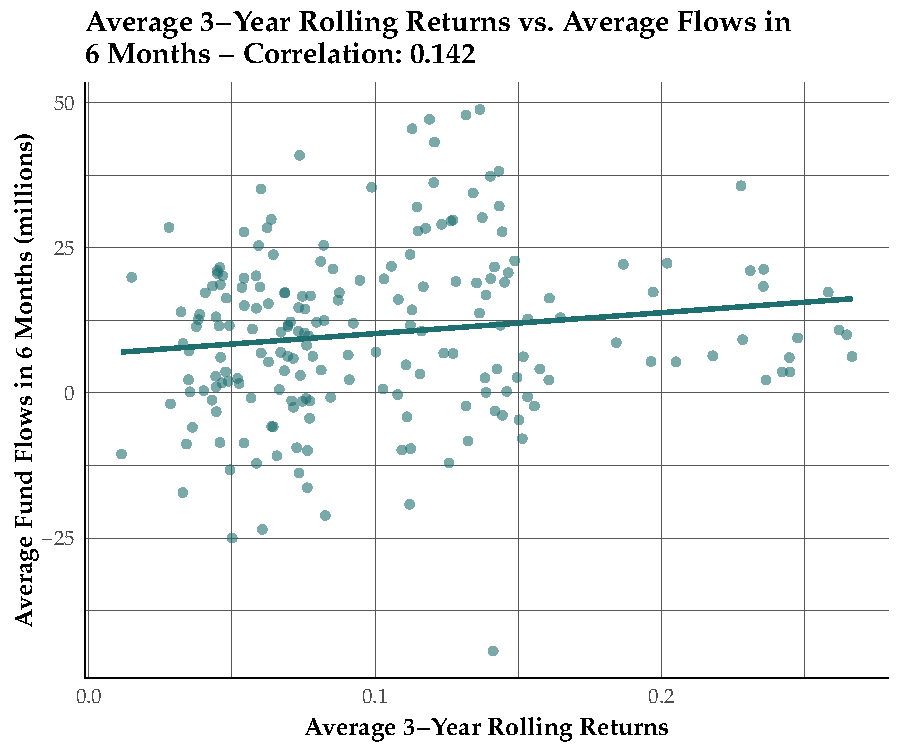
\includegraphics{Question-4_files/figure-latex/unnamed-chunk-4-1.pdf}

\hypertarget{conclusion}{%
\section{Conclusion}\label{conclusion}}

Based on the results presented, it appears that there is a positive
relationship between the past performance of funds, as measured by
3-year rolling returns, and future fund inflows, albeit this
relationship is relatively weak. While top-performing funds tend to
attract more inflows, the influence of past performance on future flows
diminishes over time, becoming negligible at the 3-year mark. The
variability in fund flows suggests that factors beyond past returns play
a significant role in investment decisions. Overall, while past
performance may offer some indication of future fund attractiveness, it
should not be solely relied upon for investment decisions. Investors and
fund managers should consider a wider range of factors when evaluating
fund performance and investor behavior.

\bibliography{Tex/ref}





\end{document}
